\documentclass[10pt, letterpaper]{article}

% ============================================================
% SHANNON HOMAGE STYLE — 2-page compact
% Bell System Technical Journal, 1948
% ============================================================

\usepackage[T1]{fontenc}
\usepackage{mathpazo}
\usepackage[scaled=0.85]{helvet}
\usepackage{microtype}
\usepackage{geometry}
\usepackage{booktabs}
\usepackage{array}
\usepackage{tikz}
\usepackage{fancyhdr}
\usepackage{titlesec}
\usepackage{enumitem}
\usepackage{xcolor}
\usepackage{multicol}
\usepackage{hyperref}

% --- Tight geometry ---
\geometry{
  letterpaper,
  top=0.75in,
  bottom=0.7in,
  left=1.0in,
  right=1.0in
}

% --- Colors ---
\definecolor{rule}{gray}{0.3}
\definecolor{lightgray}{gray}{0.55}
\definecolor{tablegray}{gray}{0.95}

\hypersetup{
  colorlinks=false,
  pdfborder={0 0 0},
  pdftitle={VSOS: The Receipt},
  pdfauthor={Faraday1, JARVIS}
}

% --- Headers ---
\pagestyle{fancy}
\fancyhf{}
\renewcommand{\headrulewidth}{0.4pt}
\fancyhead[L]{\footnotesize\textit{VibeSwap Research}}
\fancyhead[R]{\footnotesize\textit{April 2026}}
\fancyfoot[C]{\footnotesize\thepage}

% --- Compact sections ---
\titleformat{\section}
  {\normalsize\bfseries\scshape}
  {\thesection.}{0.4em}{}
  [\vspace{1pt}\titlerule]

\titlespacing*{\section}{0pt}{0.9em}{0.4em}

% --- Tight paragraph spacing ---
\setlength{\parindent}{0pt}
\setlength{\parskip}{0.35em}

% --- Tight lists ---
\setlist{nosep, leftmargin=1.2em, topsep=0pt, partopsep=0pt}

% --- Custom commands ---
\newcommand{\thinrule}{\vspace{2pt}\noindent\textcolor{rule}{\rule{\textwidth}{0.4pt}}\vspace{2pt}}
\newcommand{\sub}[1]{\textbf{#1}\enspace}

\begin{document}

% ============================================================
% TITLE BLOCK — compact
% ============================================================

\begin{center}
  \vspace*{-0.1in}

  {\Large\bfseries VSOS: The Receipt}%
  \hspace{1em}{\normalsize We Built the Whole Thing}

  \vspace{4pt}
  \textcolor{rule}{\rule{4in}{0.5pt}}
  \vspace{4pt}

  {\small\textsc{Faraday1} \enspace\&\enspace \textsc{JARVIS}%
  \quad$\cdot$\quad \textit{VibeSwap Research}%
  \quad$\cdot$\quad \textcolor{lightgray}{April 2026}}

  \vspace{0.15in}
\end{center}

% ============================================================
% CHANNEL DIAGRAM — compact Shannon tell
% ============================================================

\begin{center}
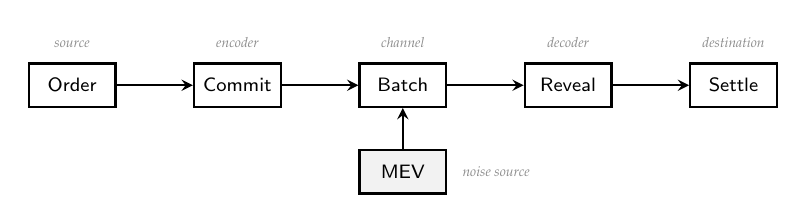
\begin{tikzpicture}[
  box/.style={draw, thick, minimum width=1.1cm, minimum height=0.55cm, font=\scriptsize\sffamily},
  arr/.style={->, thick, >=stealth},
  lbl/.style={font=\tiny\itshape, text=lightgray}
]
  \node[box] (src)  at (0,0)    {Order};
  \node[box] (enc)  at (2.1,0)  {Commit};
  \node[box] (chan) at (4.2,0)  {Batch};
  \node[box] (dec)  at (6.3,0)  {Reveal};
  \node[box] (dst)  at (8.4,0)  {Settle};

  \draw[arr] (src) -- (enc);
  \draw[arr] (enc) -- (chan);
  \draw[arr] (chan) -- (dec);
  \draw[arr] (dec) -- (dst);

  \node[lbl, above=2pt] at (src.north)  {source};
  \node[lbl, above=2pt] at (enc.north)  {encoder};
  \node[lbl, above=2pt] at (chan.north) {channel};
  \node[lbl, above=2pt] at (dec.north)  {decoder};
  \node[lbl, above=2pt] at (dst.north)  {destination};

  \node[box, fill=tablegray] (noise) at (4.2,-1.1) {MEV};
  \draw[arr] (noise) -- (chan);
  \node[lbl, right=2pt] at (noise.east) {noise source};
\end{tikzpicture}
\end{center}

\vspace{0.05in}

% ============================================================
% 1. THE CLAIM
% ============================================================

\section{The Claim}

VibeSwap is not a whitepaper. It is a financial operating system---designed, implemented, tested, and hardened. Every mechanism described in our research papers exists as deployed Solidity. This document is the proof.

% ============================================================
% 2. BY THE NUMBERS
% ============================================================

\section{By the Numbers}

\vspace{-0.2em}
\begin{center}
\small
\begin{tabular}{@{} l r @{\qquad} l r @{}}
\toprule
Solidity contracts & 385 & RSI audit cycles & 6 \\
Test functions & 10{,}559 & TRP rounds & 53 \\
Lines of Solidity & 114{,}762 & Critical vulns found \& fixed & 14+ \\
Contract directories & 31 & Regressions after fixes & 0 \\
\bottomrule
\end{tabular}
\end{center}

% ============================================================
% 3. THE ARCHITECTURE
% ============================================================

\section{The Architecture}

Seven layers, one system. Shared interfaces throughout. One oracle, one settlement engine, one security model.

\vspace{0.2em}
\begin{center}
\small
\renewcommand{\arraystretch}{1.15}
\begin{tabular}{@{} c @{\;\;} l @{\;\;} l @{}}
\toprule
& \textbf{Layer} & \textbf{Components} \\
\midrule
\textsf{\textbf{7}} & \textsc{Cross-Chain} & LayerZero V2 OApp, omnichain messaging \\
\textsf{\textbf{6}} & \textsc{Identity} & Soulbound IDs, AI agent registry (ERC-8004), VibeCode \\
\textsf{\textbf{5}} & \textsc{Framework} & Hook registry, plugin lifecycle, version router \\
\textsf{\textbf{4}} & \textsc{Governance} & Conviction voting, quadratic voting, commit-reveal gov \\
\textsf{\textbf{3}} & \textsc{Financial} & Options, bonds, credit, synths, insurance, streaming \\
\textsf{\textbf{2}} & \textsc{AMM} & Modular curves (constant product, StableSwap, custom) \\
\textsf{\textbf{1}} & \textsc{Core} & Commit-reveal batch auctions, circuit breakers, TWAP \\
\bottomrule
\end{tabular}
\end{center}

% ============================================================
% 4. WHAT'S IMPLEMENTED — dense inline format
% ============================================================

\section{What's Implemented}

\sub{Core Settlement.} Commit-reveal batch auctions with 10-second cycles (8s commit, 2s reveal). Fisher-Yates deterministic shuffle using XORed participant secrets. Uniform clearing price---every order in a batch gets the same price. Flash loan protection (EOA-only commits). 50\% slashing for invalid reveals. TWAP validation (max 5\% deviation).

\sub{AMM.} Constant product ($x \cdot y = k$) and StableSwap curves. Pluggable curve interface (\texttt{IPoolCurve}). Permissionless pool creation via factory. PID-controlled fee adjustment.

\sub{Financial Primitives.} 11 built-in applications: options, bonds, credit, synthetics, insurance, LP NFTs, streaming, revenue sharing, prediction markets, bonding curve launches, wrapped batch auction receipts. All sharing the same oracle, settlement, and security infrastructure.

\sub{Security.} Five independent defense layers: (1)~MEV elimination via commit-reveal, (2)~oracle validation (TWAP + Kalman filter), (3)~circuit breakers (volume, price, withdrawal), (4)~rate limiting (100K tokens/hour/user), (5)~extension sandboxing (500K gas cap, non-reverting).

\sub{Governance.} Conviction voting, quadratic voting, commit-reveal governance, retroactive funding, on-chain forum, decentralized tribunal. Treasury stabilizer with automatic rebalancing.

\sub{Identity.} Soulbound identity, ERC-8004 agent registry, context anchoring, pairwise verification (CRPC), unified VibeCode fingerprint.

\sub{Extensibility.} Hooks at 6 injection points (gas-limited, non-reverting). Full plugin lifecycle (proposed $\to$ approved $\to$ grace period $\to$ active $\to$ deprecated). Version router with opt-in upgrades and parallel version operation.

\sub{Three-Token Consensus.} \textbf{VIBE} (Proof of Mind)---governance, earned through contribution. \textbf{JUL} (Proof of Work)---compute rewards, mined by AI agents. \textbf{CKBn} (Proof of Stake)---bridged CKB, economic security. Constitutional separation of powers. Tinbergen's Rule: one instrument per policy objective.

\sub{Cross-Chain.} LayerZero V2 integration. Omnichain swaps, liquidity migration, cross-chain governance.

% ============================================================
% 5. HOW WE BUILT IT
% ============================================================

\section{How We Built It}

Two people and an AI. The entire codebase was developed using \textbf{TRP} (Test-Repair Protocol)---a recursive self-improvement methodology. Each round: audit, classify by severity, fix, verify zero regressions, repeat. 53 rounds. Every round tightened the system.

The AI (JARVIS) is a development partner operating under protocol constraints---anti-hallucination checks, citation hygiene, crash recovery, session state persistence. The methodology itself is a research contribution: production-grade systems with AI assistance under real hardware constraints (6-core CPU, 16GB RAM). Six full RSI cycles produced 14+ critical fixes and 0 regressions. The test suite grew from nothing to 10{,}559 functions across 522 test files.

% ============================================================
% 6. THE TRUST SURFACE
% ============================================================

\section{The Trust Surface}

Despite 385 contracts, the critical audit surface is small: settlement correctness ($\sim$1{,}150 lines) + fund access ($\sim$885 lines) = \textbf{$\sim$2{,}035 lines}. Everything else---financial primitives, governance, hooks, plugins---runs in userspace. A bug in options cannot drain AMM pools. A malicious hook cannot alter settlement prices. Structural enforcement, not convention.

% ============================================================
% 7. WHAT THIS MEANS
% ============================================================

\section{What This Means}

Most DeFi projects publish a whitepaper and ship one contract. We published the theory (\textit{Econom\'itra}), the methodology (\textit{Symbolic Compression}), the efficiency model (\textit{AI Efficiency Trinity})---and then we built the entire system those papers describe. 385 contracts. 10{,}559 tests. 7 layers. 3 tokens. 0 regressions.

The papers are the blueprint. This is the building.

\thinrule

\begin{center}
  \textcolor{lightgray}{\footnotesize\textit{Source:} \texttt{github.com/wglynn/vibeswap}}
\end{center}

\end{document}
